\documentclass[a4paper, 12pt]{article}

\usepackage[english]{babel}
\usepackage{parskip}
\usepackage[shortlabels]{enumitem}
\usepackage{amsmath,amsfonts}
\usepackage{listings}
\usepackage[margin=1.5cm]{geometry}
\usepackage{graphicx}
\usepackage{chemformula}
\usepackage{subfig}
\usepackage{siunitx}
\usepackage{microtype}


\usepackage{xcolor}
\newcommand*\circled[1]{\kern-2.5em%
  \put(0,4){\color{red}\circle*{18}}\put(0,4){\circle{16}}%
  \put(-4,0){\color{white}\bfseries\large#1}~~}
\usepackage{enumitem}

\usepackage{hyperref}
\hypersetup{
    colorlinks=true,
    urlcolor=red,
    linkcolor=black,
    urlcolor=blue,
    linkbordercolor= 1 1 1,
    urlbordercolor=1 1 1,
    }
\usepackage{cleveref}
\crefformat{footnote}{#2\footnotemark[#1]#3}

\title{PyES User Manual}
\date{v1.0.0}

\begin{document}
\maketitle

\tableofcontents

\clearpage
\newpage

\section{Introduction}
PyES is a software for the computation of species concentration at equilibrium.
This manual wants to be a quick start guide for the end user, allowing to get accustomed to the interface as possible.
If interested in the math behind the calculations it would be more of interest to read \href{https://papers.ssrn.com/sol3/papers.cfm?abstract_id=4375932}{\underline{the paper}}.


This manual is organized as follows:
\begin{itemize}[\textbullet]
    \item Section \ref*{sec:glossary} introduces some of the common terminology used throughout this document.
    \item Section \ref*{sec:installation} briefly guides through the installation process for the supported platforms.
    \item Section \ref*{sec:interface} presents the software interface and explains the meaning of the various input fields available to the user.
    \item Section \ref*{sec:examples} provides examples of the various work modes of the software.
\end{itemize}

\newpage

\section{Glossary}
\label{sec:glossary}
\textbf{Chemical System:} a closed chemical system which includes both liquid and solid phase.

\textbf{Species:} chemical entity present in the chemical system, it can be ``soluble'' (meaning it only resides in the liquid phase) or ``precipitable'' (it can precipitate leaving the liquid phase).

\textbf{Component:} subset of the species in the system that can be used to describe the rest through their  stoichiometric coefficients.
It is important to note that a component does not need to be a single atomic entity (i.e. \ch{H3PO4} can be defined as  3$\times$\ch{H+} + 1$\times$\ch{PO4^{3-}}, a metallic complex of glycine and copper can be written as  1$\times$\ch{Cu} + 1$\times$\ch{gly})

\textbf{Analytical Concentration:} the ``total concentration'' of a component; that is the summed molar concentration of all the species containing said component multiplied by the corresponding stoichiometric coefficient. 

\textbf{Background Ions:} chemical species that do not directly interact with the chemical system but affect the ionic strength of the solution.

\newpage

\section{Installation}
\label{sec:installation}
In this a brief explanation on how to install PyES will be provided.

PyES is compatible with any X86-64 hardware.
The following Operating System are officially supported.
\begin{itemize}[\textbullet]
    \item Windows 10+
    \item macOS 10.14+ 
    \item Ubuntu 20.04+

\end{itemize}

PyES might work on other systems but it is not guaranteed.

The various installers can be downloaded from the \href{https://github.com/Kastakin/PyES/releases/latest}{\underline{release page}} on GitHub.


\subsection{Windows}
\begin{enumerate}
    \item Double click on the downloaded \verb|.exe| installer
    \item If prompted with the request of giving permissions to modify your system click ``Yes''\footnote{\label{note1}For the time being we are not able to sign our installers, this might prompt with some security alerts on Windows and macOS. Our software does not execute any code whose purpose is other then solving solution and precipitation equilibria. We encourage to audit our code on \href{https://github.com/Kastakin/PyES}{\underline{GitHub}}}.
    \item Follow the instructions provided by the installer.
\end{enumerate}

\subsection{MacOS}
\begin{enumerate}
    \item Double click on the downloaded \verb|.dmg| file
    \item If the OS blocks the file from opening follow the \href{https://support.apple.com/it-it/guide/mac-help/mh40616/mac}{\underline{official instructions}} to open unsigned applications\cref{note1}.
    \item Follow the instructions provided by the installer.
\end{enumerate}

\subsection{Linux}
\begin{enumerate}
    \item Open a terminal
    \item Execute \verb|sudo apt install path_to_deb| where \verb|path_to_deb| points to the downloaded \verb|.deb| file on you system.
\end{enumerate}

\newpage


\section{User Interface}
\label{sec:interface}

The main interface presented to the user after launching the software can be seen in Figure \ref*{fig:main}.

\begin{enumerate}[label=\protect\circled{\arabic*}]
    \item The title bar bears the path of the current project (or ``New Project'' if the current project has not be saved yet).
    \item In the menu bar shortcuts for the most common operations are present (i.e. create/open a project, save the current project, launch a calculation, \ldots).
    \item A brief explanation of the hovered field or button is displayed in the status bar at the bottom.
\end{enumerate}

\begin{figure}[h]
	\centering
	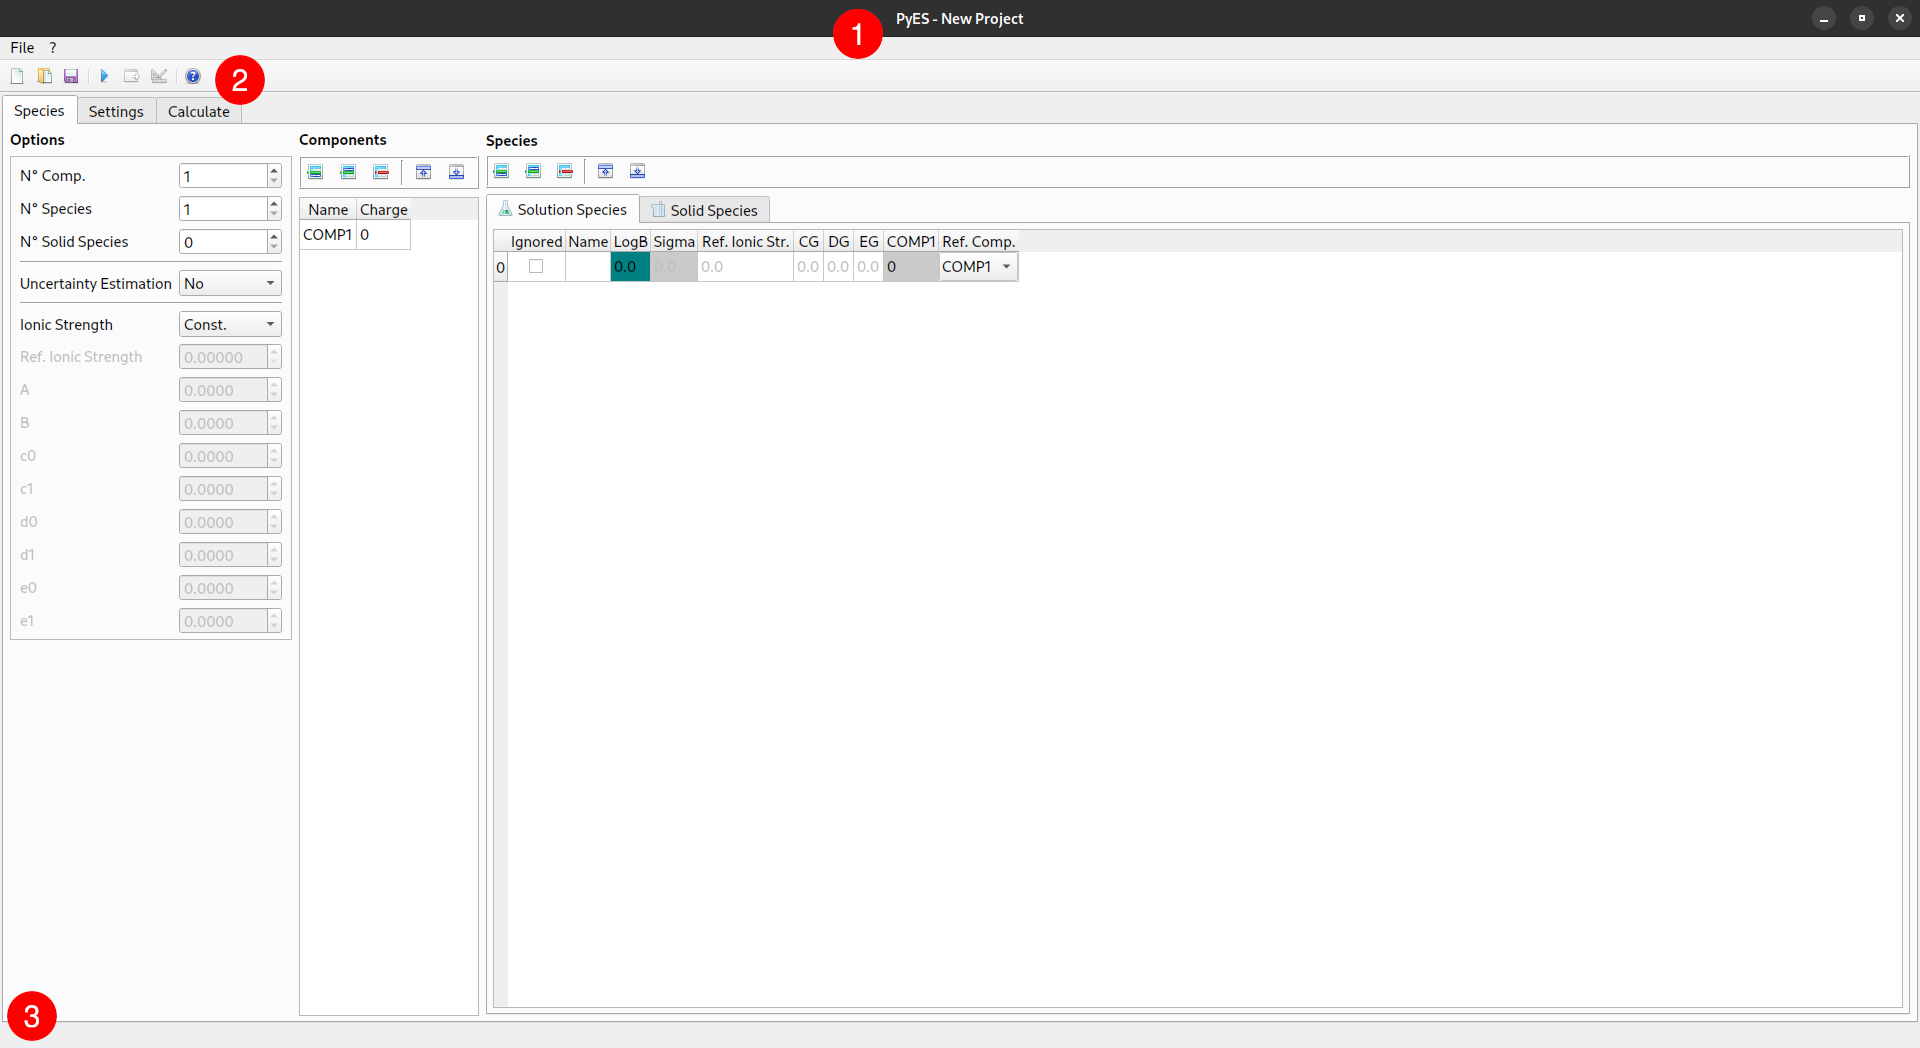
\includegraphics[width=\textwidth]{img/main.png}
	\caption{Main Window}
    \label{fig:main}
\end{figure}

The interface is organized in three main tabs, each representing a different step in the definition of the calculation parameters.

\subsection{Species Tab}
The ``Species'' tab (Figure \ref*{fig:species}) is the one shown by default to the user after opening the software for the first time.
In this tab is where a qualitative description of the chemical system is input.
In particular the interface presents the following input fields:

\begin{enumerate}[label=\protect\circled{\arabic*}]
    \item Number of components, soluble and precipitable species.
    \item Computation of ```Uncertainty Estimation'' deriving from uncertainties of inputs and effect of ionic strength on stability constants.
    \item Table for defining components names and charges.
    \item Tables to input soluble and precipitable species depending on whether the "Solution Species" or "Solid Species" pages has been selected.
    \item Quick commands to move/insert/remove species and components from their corresponding tables.
\end{enumerate}

\begin{figure}[h]
	\centering
	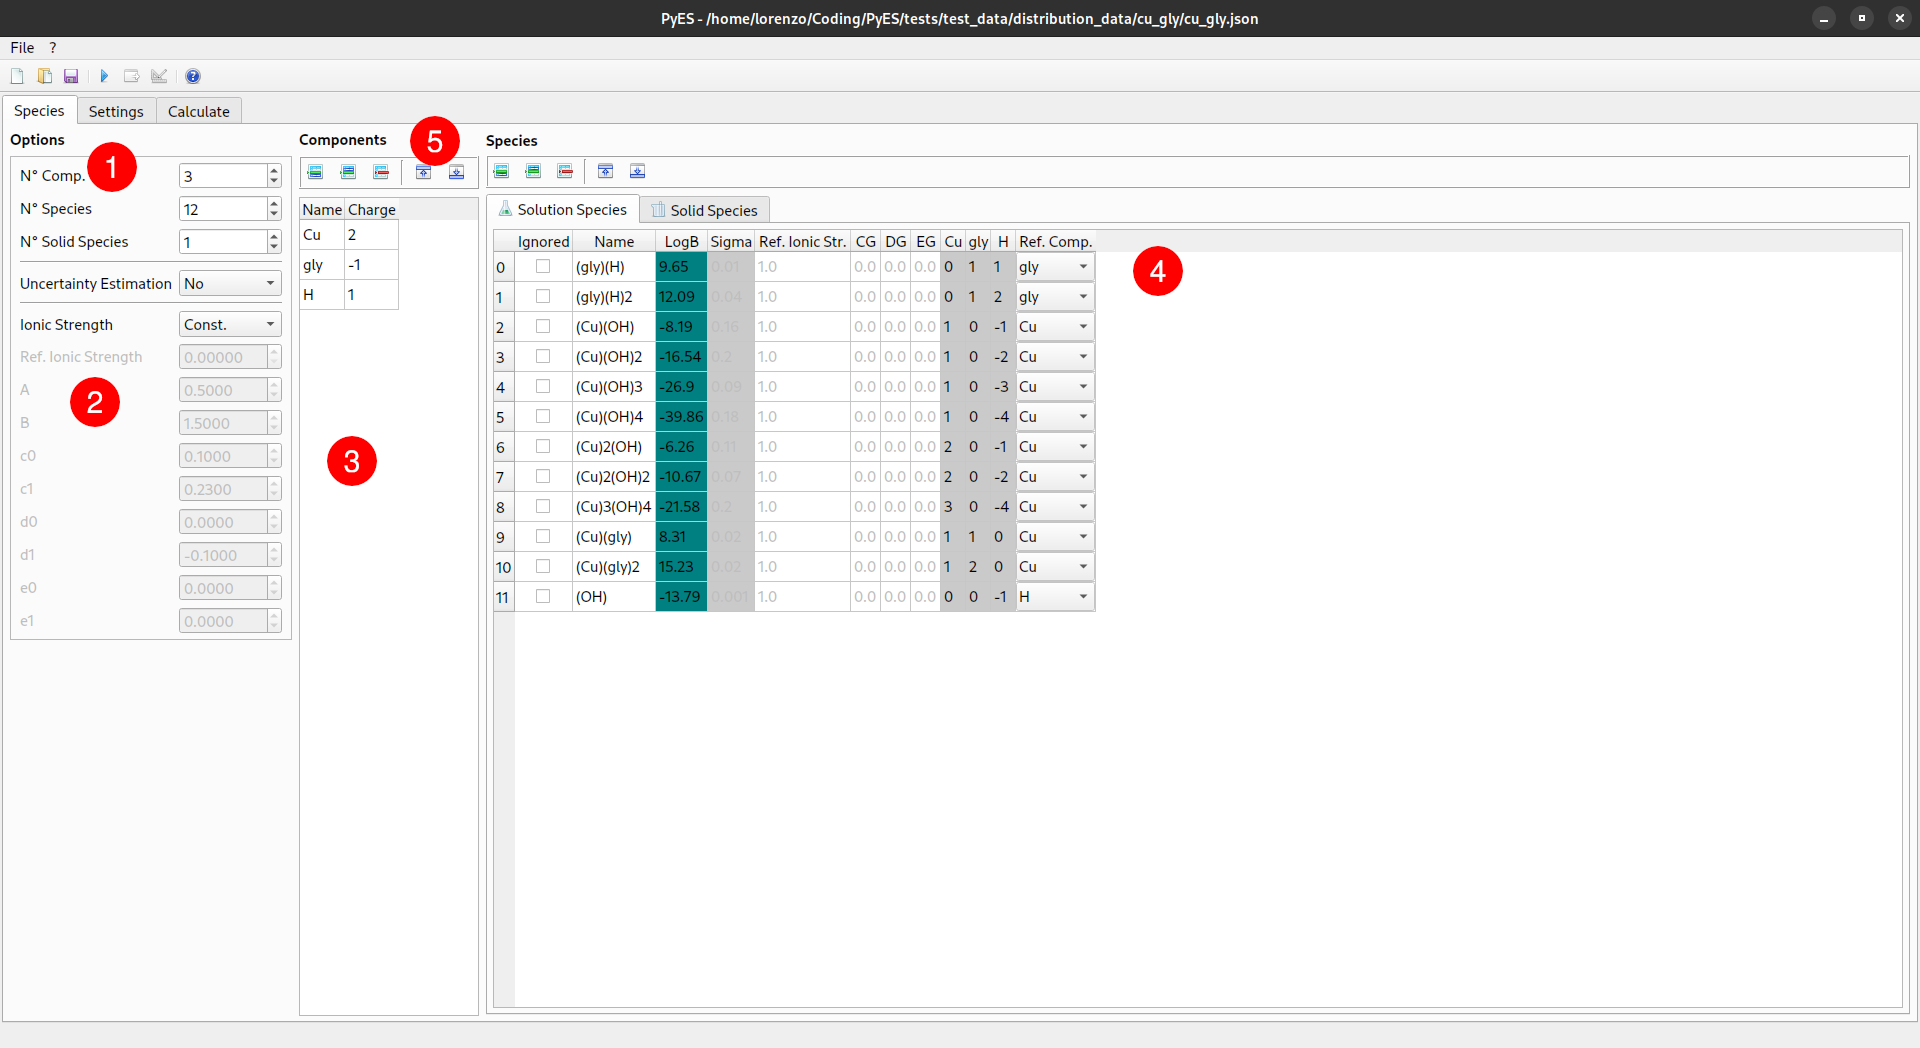
\includegraphics[width=\textwidth]{img/species.png}
	\caption{Species Tab}
    \label{fig:species}
\end{figure}

Soluble and precipitable species tables are shown in details in Figure \ref*{fig:species_tables}.
They are very similar, requiring the user to provide the following information for each one of the species present:

\begin{enumerate}[label=\protect\circled{\arabic*}]
    \item Checkbox to exclude the corresponding species from the calculation (useful to test different systems assemblages without having to create a project for each one).
    \item Name of the species; this is not an editable space, the name is obtained from the stoichiometric coefficient of the species itself.
    \item Depending on the type of species $\log_{10}$ of stability constant/solubility product of the species.
    \item Uncertainty on the stability constant/solubility product of the species, used for the propagation of uncertainty, only active when the corresponding option is selected in the ``Species'' tab.
    \item Reference ionic strength and Debye-H\"uckel parameters for which the stability constant/solubility product of the species is defined; this can be left at zero, using the project-wise values defined in the ``Species'' tab.
    \item Stoichiometric coefficients of components used to defined the species.
    \item Component to use to compute the species concentration as a fraction of analytical concentration of the component. 
\end{enumerate}

\begin{figure}[h]
    \centering
    \subfloat[\centering Soluble]{{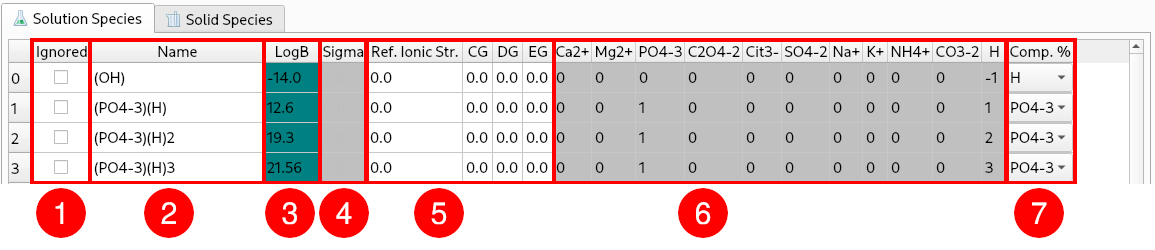
\includegraphics[width=\textwidth]{img/species_sol.png}}}%
    \qquad
    \subfloat[\centering Precipitable]{{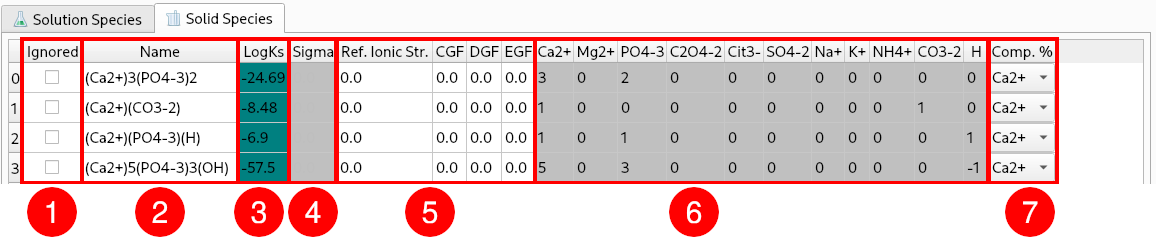
\includegraphics[width=\textwidth]{img/species_prec.png}}}%
    \caption{Species Input Tables}%
    \label{fig:species_tables}%
\end{figure}

\subsection{Settings Tab}
In the ``Setting'' tab the user can select the work mode for the calculation and provide the quantitative information of the system described in the ``Species'' tab.

\begin{figure}[h]
	\centering
	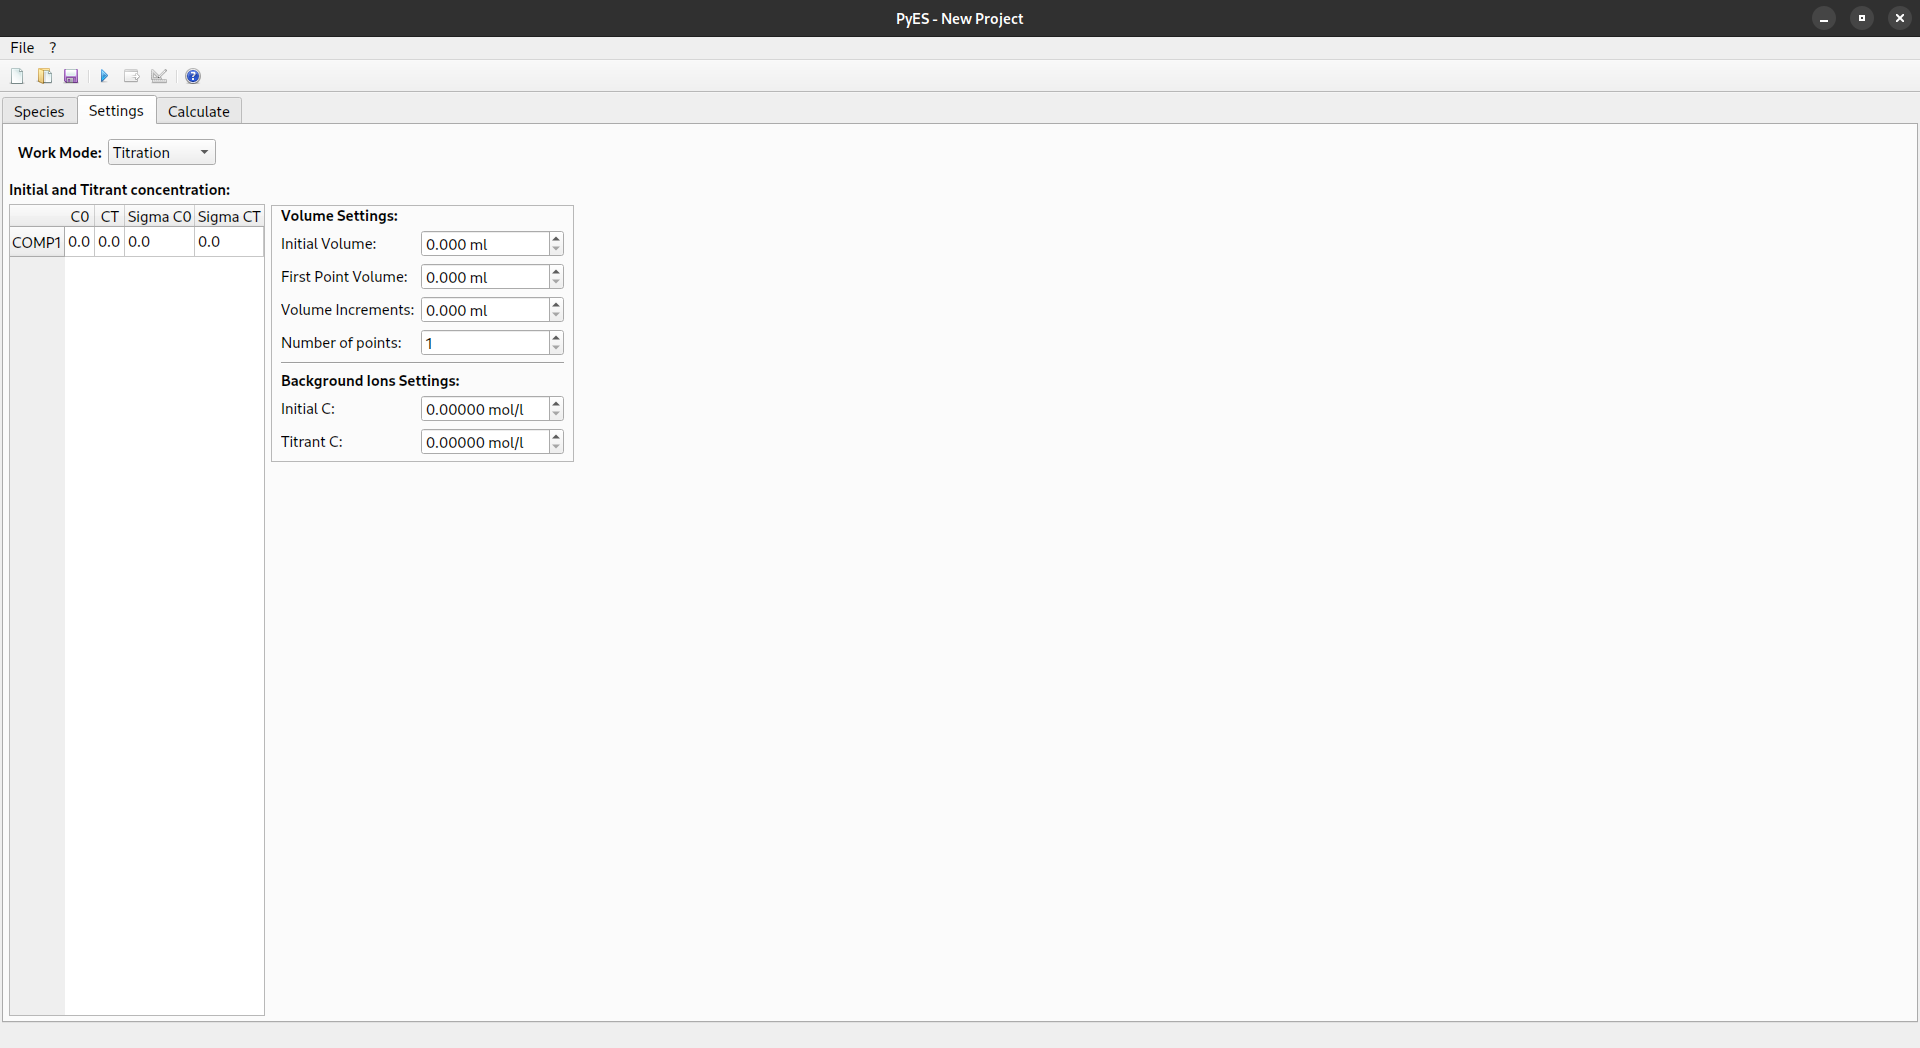
\includegraphics[width=\textwidth]{img/settings.png}
	\caption{Settings Tab}
    \label{fig:settings}
\end{figure}

Depending on the selected work mode different inputs are required from the user (Figure \ref*{fig:work_inputs}).

\subsubsection{Titration Mode}
\begin{enumerate}[label=\protect\circled{\arabic*}]
    \item Table with the analytical concentration of the components in the titration vessel (C0) and in titrant solution (CT) in \unit{\mol / \liter}; uncertainty on this values can be provided too if ``Uncertainty Estimation'' has been selected in the ``Species'' tab.
    \item Volume of titration vessel, volume at first titration point (volume of titration vessel + volume of titrant added), volume of titrant added at each titration point, number of titration points.
    \item If the effect of ionic strength has to be considered, as defined in the ``Species'' tab, the concentration of background ions in the titration vessel and in the titrant can be defined.
\end{enumerate}

\subsubsection{Distribution Mode}
\begin{enumerate}[label=\protect\circled{\arabic*}]
    \item Table with the analytical concentration of the components (C0) in \unit{\mol / \liter}; uncertainty on this values can be provided too if ``Uncertainty Estimation'' has been selected in the ``Species'' tab.
    \item Component to use as the independent one, its initial, final and increment values; changing the component disables its row in the concentration tables since it will not be used for calculation purposes.
    \item If the effect of ionic strength has to be considered, as defined in the ``Species'' tab, the concentration of background ions can be defined.
\end{enumerate}

\begin{figure}[h]%
    \centering
    \subfloat[\centering Titration]{{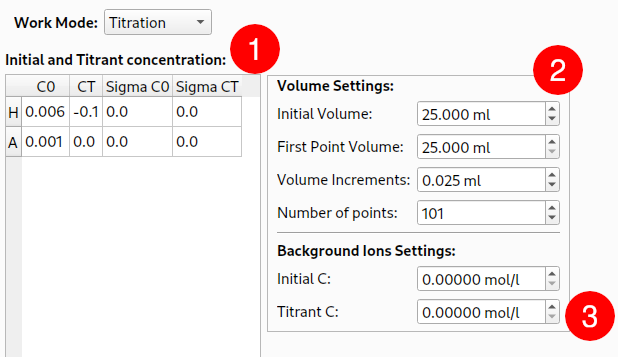
\includegraphics[width=0.4\textwidth]{img/settings_titr.png}}}%
    \qquad
    \subfloat[\centering Distribution]{{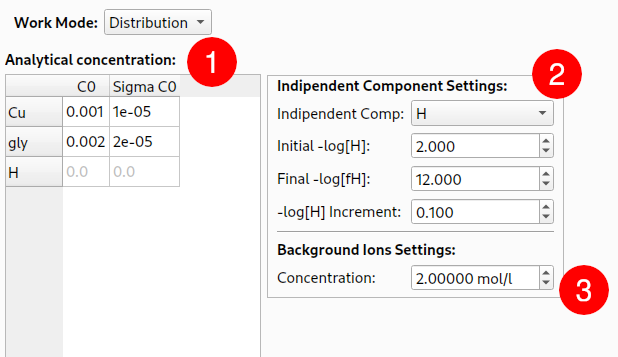
\includegraphics[width=0.4\textwidth]{img/settings_dist.png}}}%
    \caption{Different Work Mode Inputs}%
    \label{fig:work_inputs}%
\end{figure}

\subsection{Calculate Tab}
The ``Calculation'' tab (Figure \ref{fig:calculate}) is reserved to calculation launching and reporting

\begin{enumerate}[label=\protect\circled{\arabic*}]
    \item The text box in the center is where results and uncertainties are reported in textual form to the user.
    \item Buttons dedicated to starting the calculation, exporting results and showing results in graphical form.
    \item Toggle to allow writing a log file for debugging purposes.
\end{enumerate}

\begin{figure}[h]
	\centering
	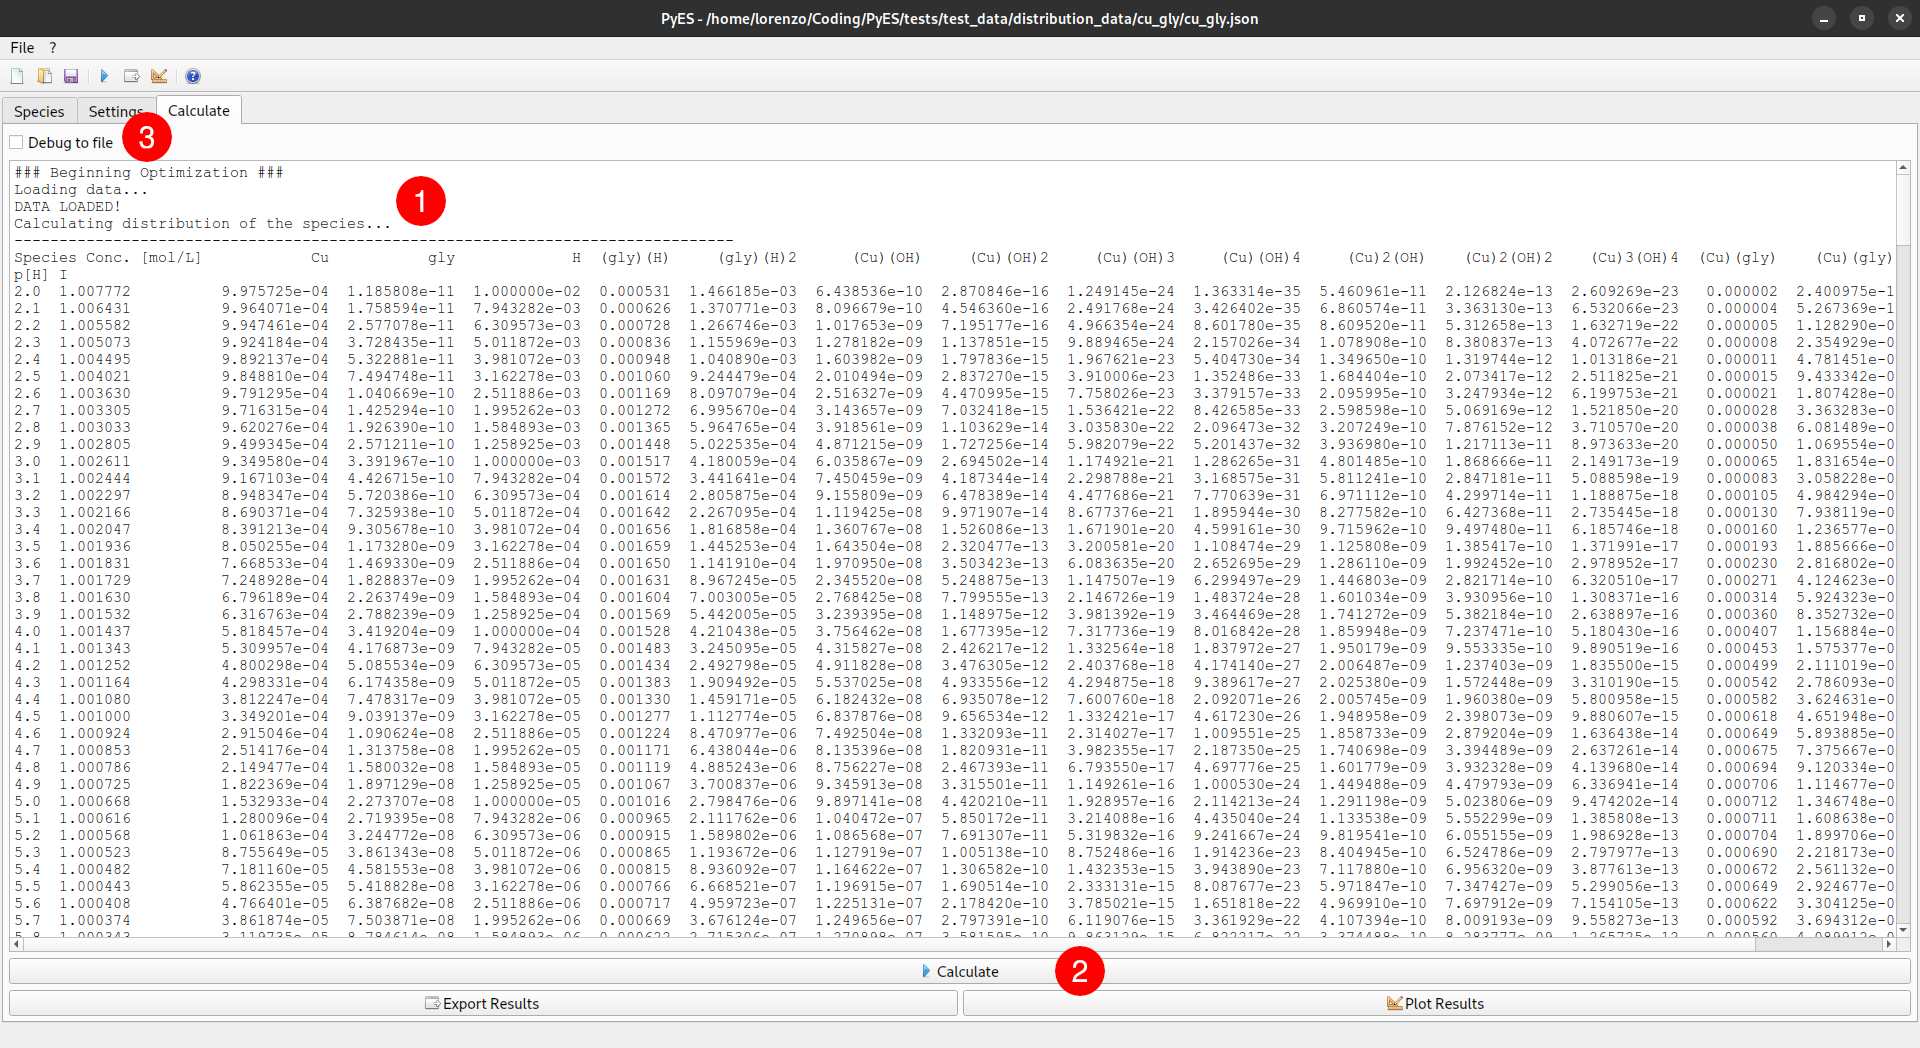
\includegraphics[width=\textwidth]{img/calculate.png}
	\caption{Calculate Tab}
    \label{fig:calculate}
\end{figure}

\subsection{Other Windows}

After a successful calculation, using the dedicated buttons in the menu bar or the ones at the bottom of the calculation tab, it is possible to access other windows for the export and the graphical output of obtained results (Figure \ref*{fig:other_windows}).

\subsubsection{Export Window}
\begin{enumerate}[label=\protect\circled{\arabic*}]
    \item The tabs allow to select if the results have to be exported as a single Excel spreadsheet or as multiple CSV files.
    \item Using the checkboxes it is possible to select only the desired results to be exported; some options may be grayed-out if the corresponding results have not being calculated (i.e. recalculated stability constants if the effect of ionic strength has not been considered).
    \item The ``Export'' button let the user pick where to save the results.
\end{enumerate}

\subsubsection{Plot Window}
\begin{enumerate}[label=\protect\circled{\arabic*}]
    \item The tabs allow to select the type of plot shown (concentration or percentages relative to components as defined in the tables in the ``Species'' tab).
    \item The plot itself; the legend can be moved by dragging it around with the mouse; right-clicking on the plot allow to change some options (i.e. axis scale, scaling, exporting as image, \ldots).
    \item The table on the left lists all the soluble and precipitable species in two different tabs; ticking/unticking any species allow to display/hide them; clicking the colored square on the right of each species name it is possible to change the color used to plot it.
    \item The buttons allow to select/deselect all the species and, clicking the ``Filter'' button, to select only the ones that contains a particular component; it is also possible, using the chekbox present to show the intervals of precipitation formation instead of the concentration of precipitates in the plot.
\end{enumerate}

\begin{figure}[h]%
    \centering
    \subfloat[\centering Export]{{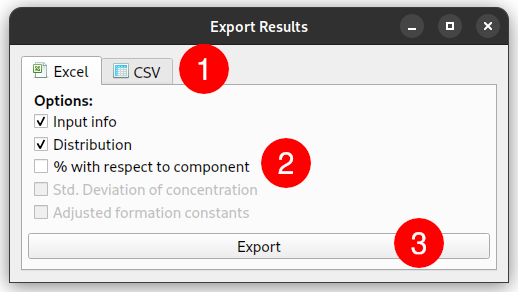
\includegraphics[width=0.4\textwidth]{img/export.png}}}%
    \qquad
    \subfloat[\centering Plot]{{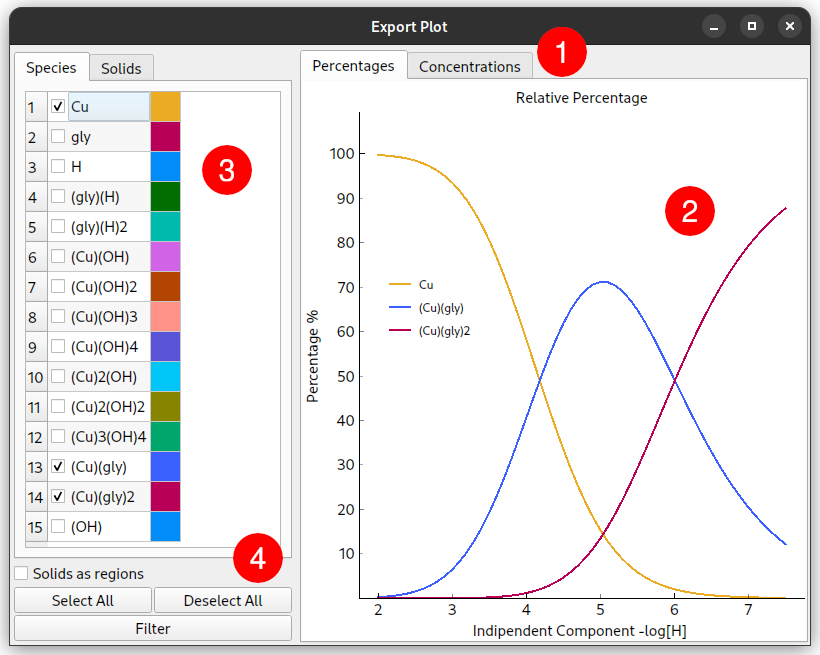
\includegraphics[width=0.4\textwidth]{img/plot.png}}}%
    \caption{Other Windows}%
    \label{fig:other_windows}%
\end{figure}

\clearpage
\newpage

\section{Examples}
\label{sec:examples}

In the following sections examples for the various work modes available in the software will be provided.
The project files used can be found in the corresponding \href{https://github.com/Kastakin/PyES/tree/master/tests/test_data}{\underline{`test' folders}} in the official GitHub page.

\subsection{Species Distribution (Cu-gly System)}
The Cu-gly system as defined by IUPAC will be used to demonstrate the computation of species distributions.

\begin{enumerate}
    \item Create a new PyES project.
    \item Define a System of 3 components, 12 soluble species and 1 precipitable species.
    \item Modify the components table to reflect the one shown in Table \ref*{tab:comp_cu_gly}.
    \item Modify the soluble species table to reflect the one shown in Table \ref*{tab:species_cu_gly}.
    \item Modify the precipitable species table to reflect the one shown in Table \ref*{tab:precipitate_cu_gly}.
    \item In the ``Settings'' tab select ``Distribution'' as the ``Work Mode''.
    \item Select ``H'' as the independent component.
    \item Define the range of $-\log_{10}H$ from $2.0$ to $12.0$ with intervals of $0.100$.
    \item Modify the ``Analytical concentration'' table, setting C0 for $\ch{Cu} = 0.001$ and  $\ch{gly} = 0.002$
    \item In the ``Calculate'' tab press the ``Calculate'' button at the bottom.
    \item Wait the pop-up reporting the termination of the calculation.
    \item Access the results in textual form from the text box in the middle, in graphical form clicking the ``Plot Results'' button at the bottom, or export them clicking the ``Export Results'' button and following the instructions.
\end{enumerate}

\begin{table}[h!]
\centering
\begin{tabular}{|l|l|}
    \hline
    \textbf{Name} & \textbf{Charge} \\ \hline
    Cu   & 2      \\ \hline
    gly  & -1     \\ \hline
    H    & 1      \\ \hline
\end{tabular}
\caption{Components Table Cu-gly}
\label{tab:comp_cu_gly}
\end{table}

\begin{table}[h!]
\centering
\begin{tabular}{|l|l|l|l|}
\hline
    \textbf{LogB}   & \textbf{Cu} & \textbf{gly} & \textbf{H}  \\ \hline
    9.65   & 0  & 1   & 1  \\ \hline
    12.09  & 0  & 1   & 2  \\ \hline
    -8.19  & 1  & 0   & -1 \\ \hline
    -16.54 & 1  & 0   & -2 \\ \hline
    -26.9  & 1  & 0   & -3 \\ \hline
    -39.86 & 1  & 0   & -4 \\ \hline
    -6.26  & 2  & 0   & -1 \\ \hline
    -10.67 & 2  & 0   & -2 \\ \hline
    -21.56 & 3  & 0   & -4 \\ \hline
    8.31   & 1  & 1   & 0  \\ \hline
    15.23  & 1  & 2   & 0  \\ \hline
    -13.79 & 0  & 0   & -1 \\ \hline
\end{tabular}
\caption{Soluble Species Table Cu-gly}
\label{tab:species_cu_gly}
\end{table}

\begin{table}[h!]
\centering
\begin{tabular}{|l|l|l|l|}
\hline
    \textbf{LogKs} & \textbf{Cu} & \textbf{gly} & \textbf{H}  \\ \hline
    8.91  & 1  & 0   & -2 \\ \hline
\end{tabular}
\caption{Precipitable Species Table Cu-gly}
\label{tab:precipitate_cu_gly}
\end{table}


\subsection{Titration of Generic Hexaprotic Acid}
The simulation of titration curves will be demonstrated through the definition of a generic system containing a single hexaprotic acid.

\begin{enumerate}
    \item Create a new PyES project.
    \item Define a System of 2 components, 7 soluble species and 0 precipitable species.
    \item Modify the components table to reflect the one shown in Table \ref*{tab:comp_hexa}.
    \item Modify the soluble species table to reflect the one shown in Table \ref*{tab:species_hexa}.
    \item In the ``Settings'' tab select ``Titration'' as the ``Work Mode''.
    \item Set the titration vessel and first point volumes to $25 \unit{\ml}$ (that is, the first point of the titration will have $0 \unit{\ml}$ of additional titrant added).
    \item Set the volume increments to $0.025 \unit{\ml}$ and set the number of titration points to 101.
    \item Modify the ``Analytical concentration'' table, setting C0 for $\ch{H} = 0.006$ and  $\ch{A} = 0.001$
    \item Modify the ``Analytical concentration'' table, setting CT for $\ch{H} = -0.1$ (the titrant is basic) and leaving \ch{A} to zero.
    \item In the ``Calculate'' tab press the ``Calculate'' button at the bottom.
    \item Wait the pop-up reporting the termination of the calculation.
    \item Access the results in textual form from the textbox in the middle, in graphical form clicking the ``Plot Results'' button at the bottom, or export them clicking the ``Export Results'' button and following the instructions.
\end{enumerate}

\begin{table}[h!]
\centering
\begin{tabular}{|l|l|}
        \hline
        \textbf{Name} & \textbf{Charge} \\ \hline
        A   & -1      \\ \hline
        H    & 1      \\ \hline
\end{tabular}
\caption{Components Table Hexaprotic Acid}
\label{tab:comp_hexa}
\end{table}

\begin{table}[h!]
\centering
\begin{tabular}{|l|l|l|}
\hline
    \textbf{LogB}   & \textbf{Cu} & \textbf{H}  \\ \hline
    -13.77 & 0  & -1 \\ \hline
    10.0   & 1  & 1  \\ \hline
    18.0   & 1  & 2  \\ \hline
    24.0   & 1  & 3  \\ \hline
    28.0   & 1  & 4  \\ \hline
    31.0   & 1  & 5  \\ \hline
    33.0   & 1  & 6  \\ \hline   
\end{tabular}
\caption{Soluble Species Table Hexaprotic Acid}
\label{tab:species_hexa}
\end{table}

\end{document}